%%%%%%%%%%%%%%%%%%%%%%% bookchapter.tex %%%%%%%%%%%%%%%%%%%%%%%%%
%
% Springer LNCS Book Chapter — Camera-Ready Submission
% Template class: llncs.cls
% Submission: Double-blind review (author info removed)
%
%%%%%%%%%%%%%%%%%%%%%%%%%%%%%%%%%%%%%%%%%%%%%%%%%%%%%%%%%%%%%%%%%%%

\documentclass[runningheads,a4paper]{llncs}

\usepackage{amssymb}
\setcounter{tocdepth}{3}
\usepackage{graphicx}
\usepackage{url}
\usepackage{amsmath}
\usepackage{booktabs}

\newcommand{\keywords}[1]{\par\addvspace\baselineskip
\noindent\keywordname\enspace\ignorespaces#1}

\begin{document}

\mainmatter

\title{MoiraiVaR and GARCH-Autoformer: Two Volatility Forecasting Architectures Evaluated via a Risk-Sensitive MCDM Framework}

\titlerunning{Volatility Forecasting via Risk-Sensitive MCDM}

% Double-blind: author information omitted for review
\author{}
\authorrunning{}
\institute{}

\toctitle{Volatility Forecasting via Risk-Sensitive MCDM}
\tocauthor{}
\maketitle

\begin{abstract}
Standard volatility forecasting often optimises accuracy and tail-risk separately, leading to models that excel in point predictions but fail in risk calibration. This paper proposes two novel architectures: \emph{GARCH-Autoformer}, which ensembles a GJR-GARCH inductive bias with Autoformer residual learning, and \emph{MoiraiVaR}, which injects a VaR-aware pinball loss into Moirai foundation models. We evaluate them via a nine-criterion Multi-Criteria Decision-Making (MCDM) framework across 26 configurations, 9 markets, and 5 horizons. We introduce a Forecast Sanity Gate that eliminates 12 amplitude-collapsed models before ranking. Results show that under balanced weights (50:50), MoiraiVaR leads due to superior accuracy, while risk-priority weighting (30:70) favours Transformer-based models. 
\keywords{volatility forecasting; MCDM; Value-at-Risk; GARCH-Autoformer; MoiraiVaR; SAW; TOPSIS}
\end{abstract}

\section{Introduction}

Accurate volatility forecasting is essential for Value-at-Risk (VaR) estimation and capital allocation. However, minimising mean-squared error (MSE) does not guarantee dynamic tracking or well-calibrated tail-risk; models can achieve low MSE while producing flat predictions \cite{gneiting2011,patton2011}. We address three gaps: (1) Standard evaluation metrics fail to detect degenerate (flat or inverted) forecasts \cite{zeng2023}. (2) Existing frameworks do not jointly evaluate accuracy, dynamic tracking, and VaR backtesting \cite{hwang1981}. (3) VaR-aware fine-tuning for time-series foundation models like Moirai remains unexplored \cite{liu2025}. 

Our contributions are: (1)~The \textbf{GARCH-Autoformer} hybrid architecture for residual volatility learning; (2)~\textbf{MoiraiVaR}, injecting a tail-risk pinball loss into Moirai fine-tuning; (3)~A \textbf{Forecast Sanity Gate} to filter degenerate predictions; (4)~A \textbf{Risk-Sensitive MCDM Framework} (SAW and TOPSIS) to rank models comprehensively.

\section{Related Work}

\textbf{Evaluation and Backtesting:} Gneiting \cite{gneiting2011} and Patton \cite{patton2011} show that MSE and QLIKE reflect distinct loss functionals and remain robust to imperfect proxies. VaR calibration requires specific backtesting \cite{christoffersen1998,kupiec1995}.
\textbf{Degeneracy and MCDM:} Linear models often outperform Transformers by avoiding attention-induced smoothing (flat forecasts) \cite{zeng2023}. To balance conflicting metrics, TOPSIS \cite{hwang1981} and statistical dominance tests \cite{demsar2006} provide robust multi-objective ranking, motivating our framework.

\section{Methodology}

\subsection{Proposed Architectures}

\textbf{GARCH-Autoformer.} This three-stage hybrid (Fig.~\ref{fig:arch}a) fits a GJR-GARCH(1,1,1) model to obtain base forecasts $\hat{\sigma}_{\mathrm{GARCH},t}$. The standardised residuals $z_t$ are encoded by an Autoformer \cite{wu2021} (kernel size~5) to predict corrections $\hat{e}_{\mathrm{pred}}$. The final ensemble is $\hat{\sigma}_{\mathrm{final}} = \sqrt{\mathrm{Softplus}( \hat{\sigma}_{\mathrm{GARCH}}^2 + \hat{e}_{\mathrm{pred}} )}$, ensuring non-negativity. Training uses Student-t negative log-likelihood \cite{bollerslev1987}.

\textbf{MoiraiVaR.} This strategy (Fig.~\ref{fig:arch}b) fine-tunes pretrained Moirai encoders \cite{liu2025} with a tail-risk signal. Zero-padded 60-day log-returns are tokenised into four patches. The encoder output is mean-pooled and passed through an MLP to predict multi-horizon volatility. The novel VaR-aware loss combines MSE and a pinball loss at the $1\%$ tail: $\mathcal{L} = \mathrm{MSE}(\hat{\sigma}, \sigma_{\mathrm{true}}) + \lambda \cdot \mathrm{Pinball}(\mathrm{VaR}_{1\%},\,r_{h=1})$, with $\lambda{=}0.2$ and dynamic Student-t degrees-of-freedom inferred per market.

\begin{figure}[t]
\centering
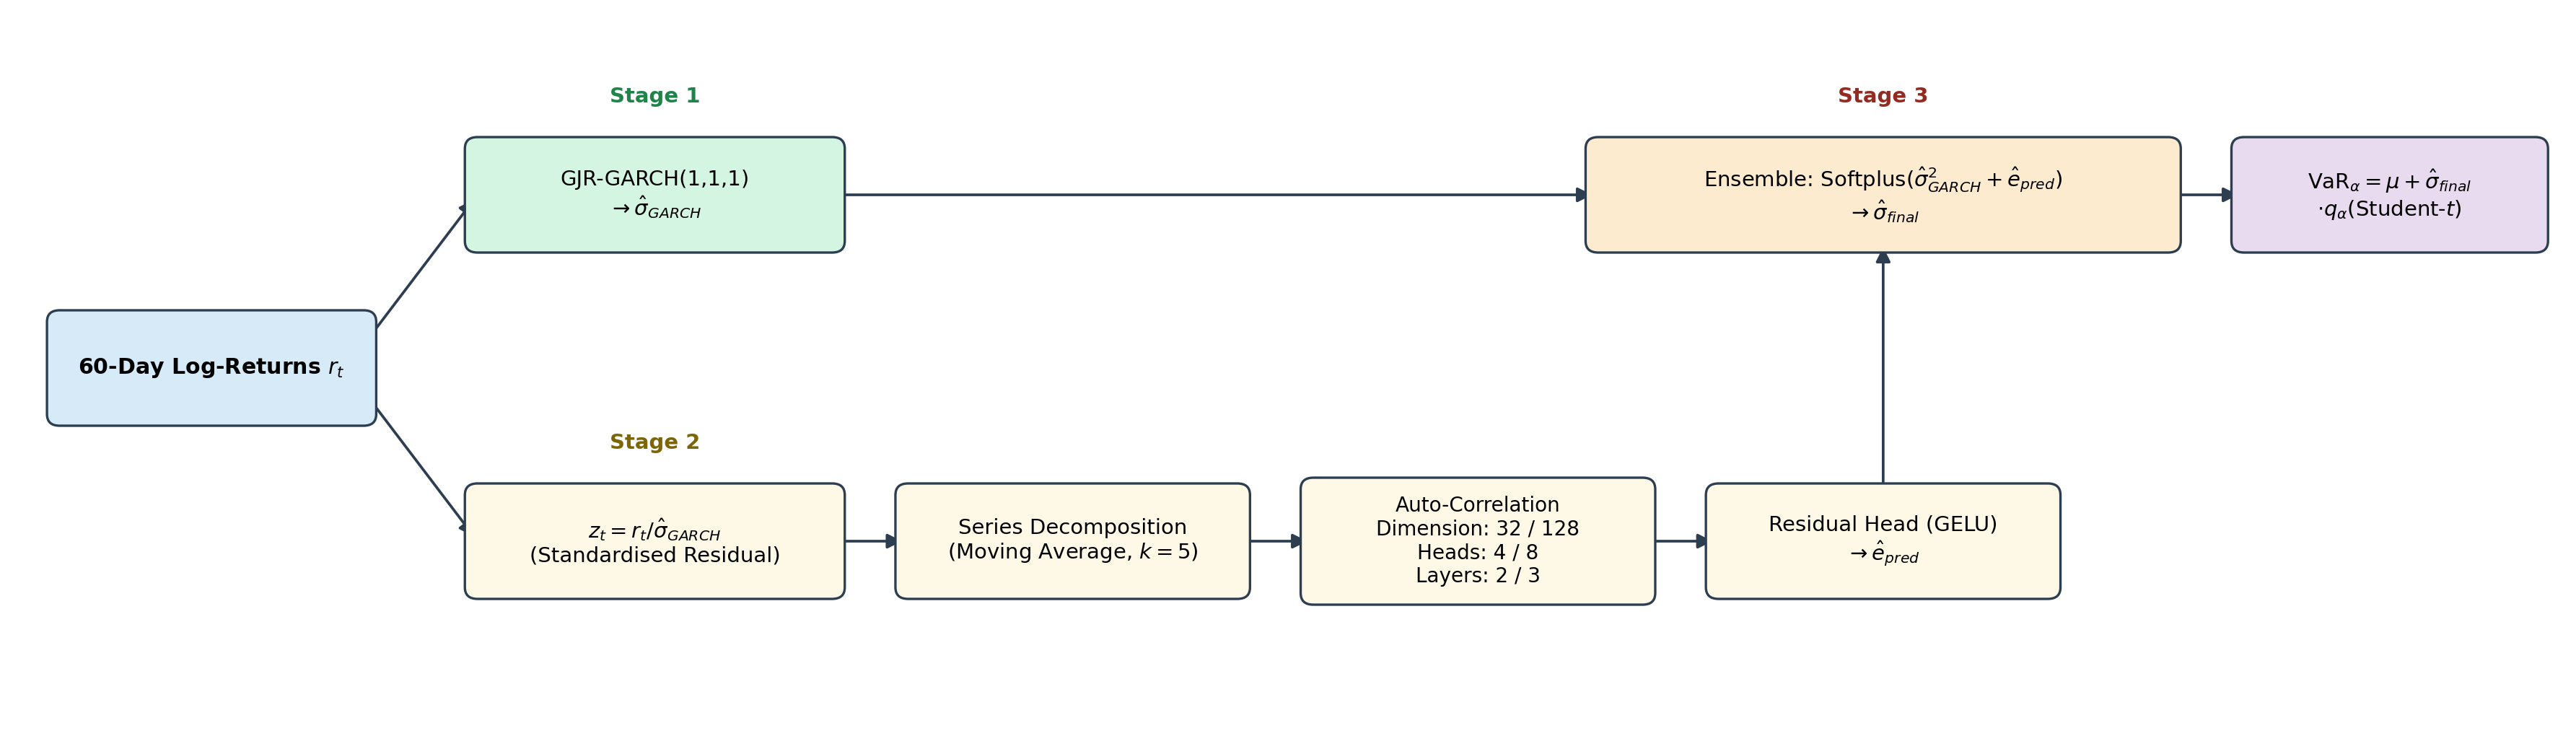
\includegraphics[width=\textwidth]{fig3a}
\vspace{0.5cm}
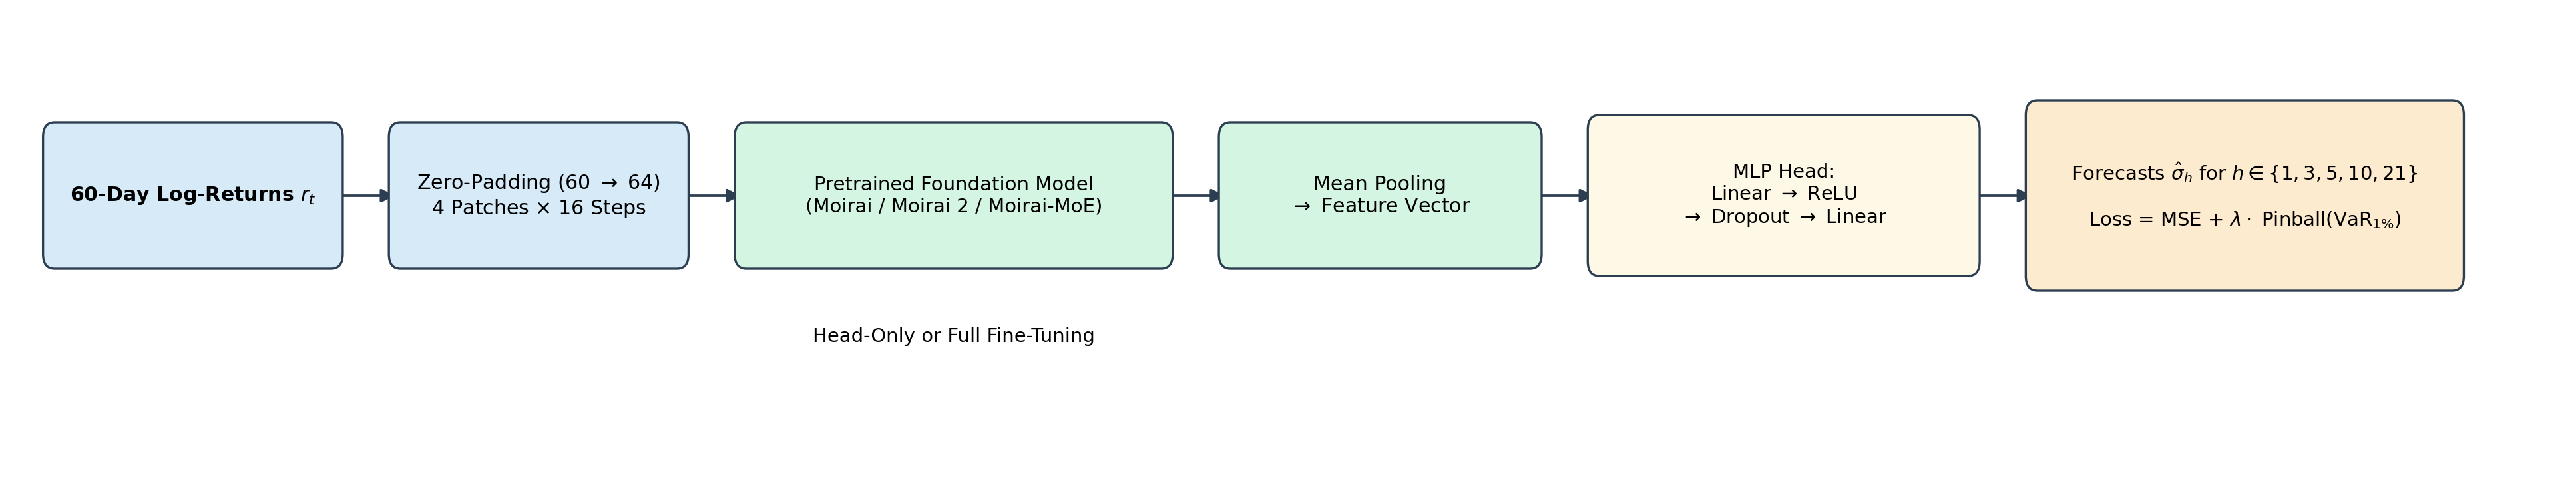
\includegraphics[width=\textwidth]{fig3b}
\caption{Architecture diagrams for the proposed (a) GARCH-Autoformer and (b) MoiraiVaR.}
\label{fig:arch}
\end{figure}

\subsection{MCDM Pipeline and Sanity Gate}

The evaluation uses nine criteria: Accuracy (MSE, MAE, QLIKE), Tracking (std-ratio error $e_\sigma$, correlation error), and Risk (VaR 1\%/5\% pass rates and average violation errors). 
Before ranking, the \textbf{Sanity Gate} eliminates models if $e_\sigma > 0.9$ (amplitude collapse) or $\rho \leq 0$ (directional inversion).
Eligible models are ranked by SAW and TOPSIS under a balanced (50:50) and a risk-priority (30:70) weight scenario.

\section{Experimental Setup}

We test 26 configurations across 16 model families on 9 market indices at 5 horizons ($h \in \{1,3,5,10,21\}$). Data is split 70\%/15\%/15\% (train/val/test).

\section{Results and Discussion}

\subsection{Raw Accuracy Comparison}

Fig.~\ref{fig:errors} compares the standalone MSE and MAE across all models prior to MCDM aggregation. Moirai-family models consistently achieve the lowest MSE and MAE, demonstrating strong point-forecast accuracy. However, pure accuracy metrics ignore tracking dynamics and tail-risk calibration.

\begin{figure}[t]
\centering
\begin{minipage}{0.48\textwidth}
  \centering
  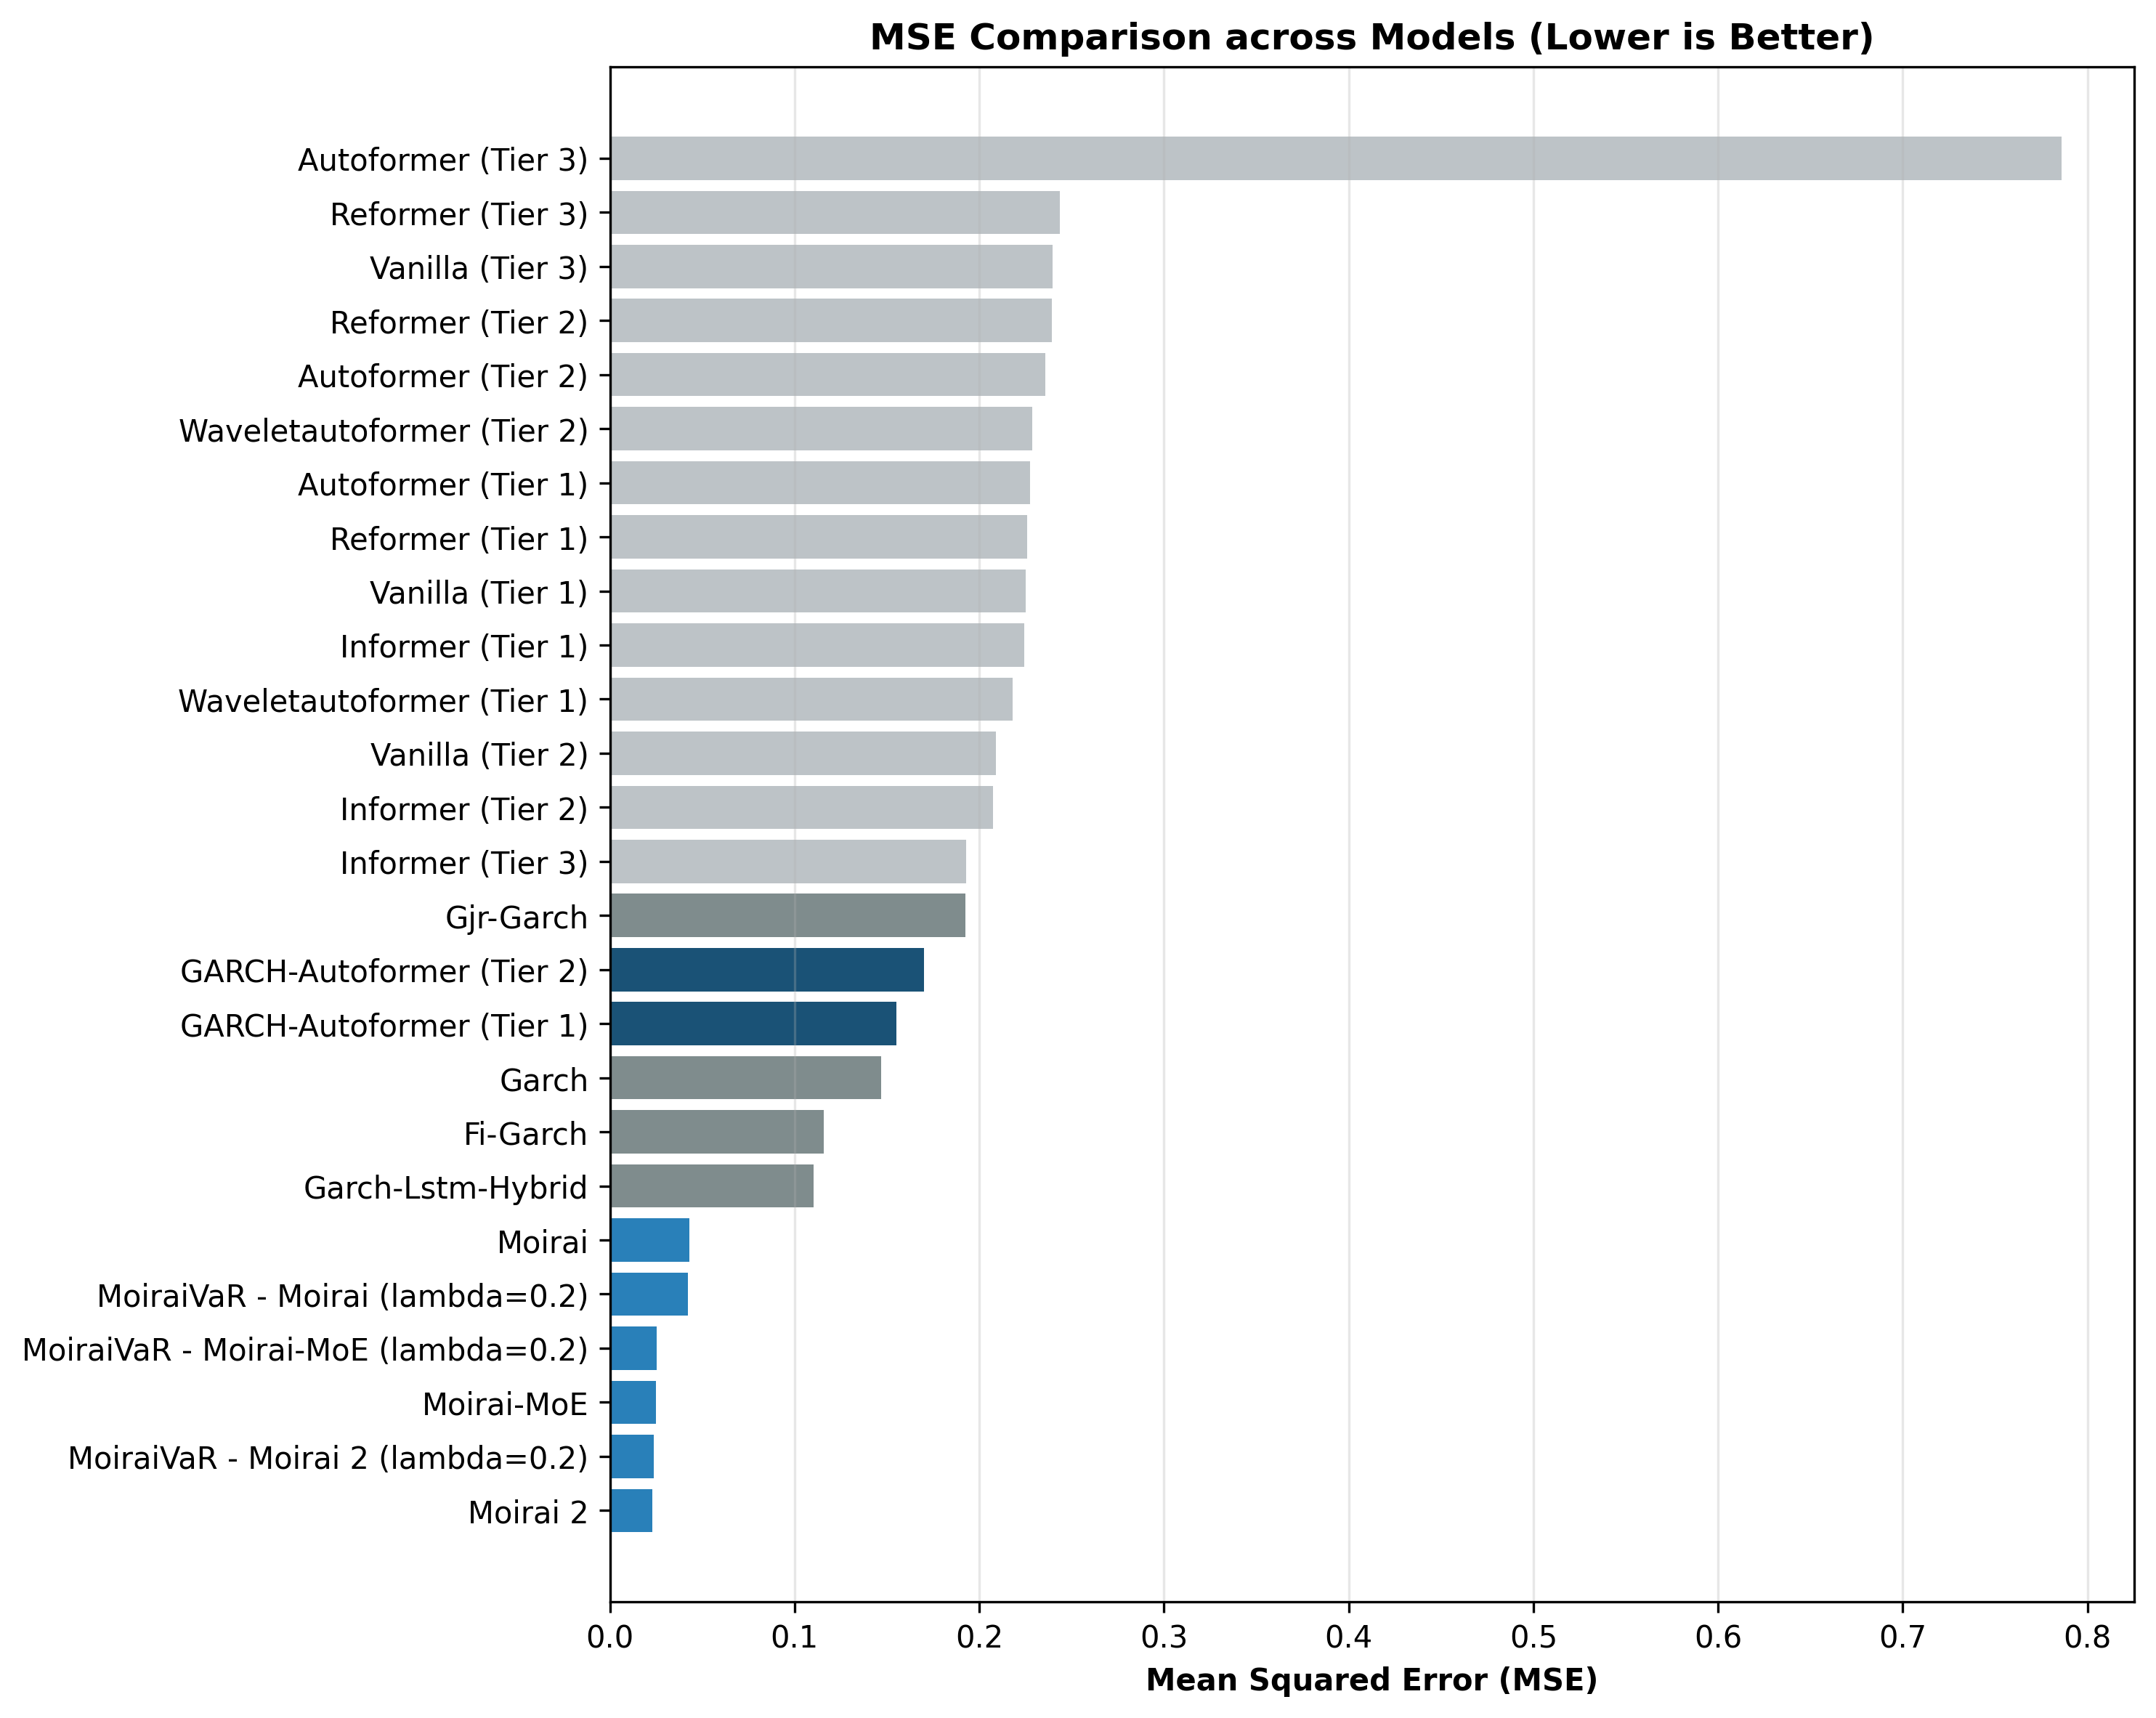
\includegraphics[width=\linewidth]{fig_mse_comparison}
\end{minipage}\hfill
\begin{minipage}{0.48\textwidth}
  \centering
  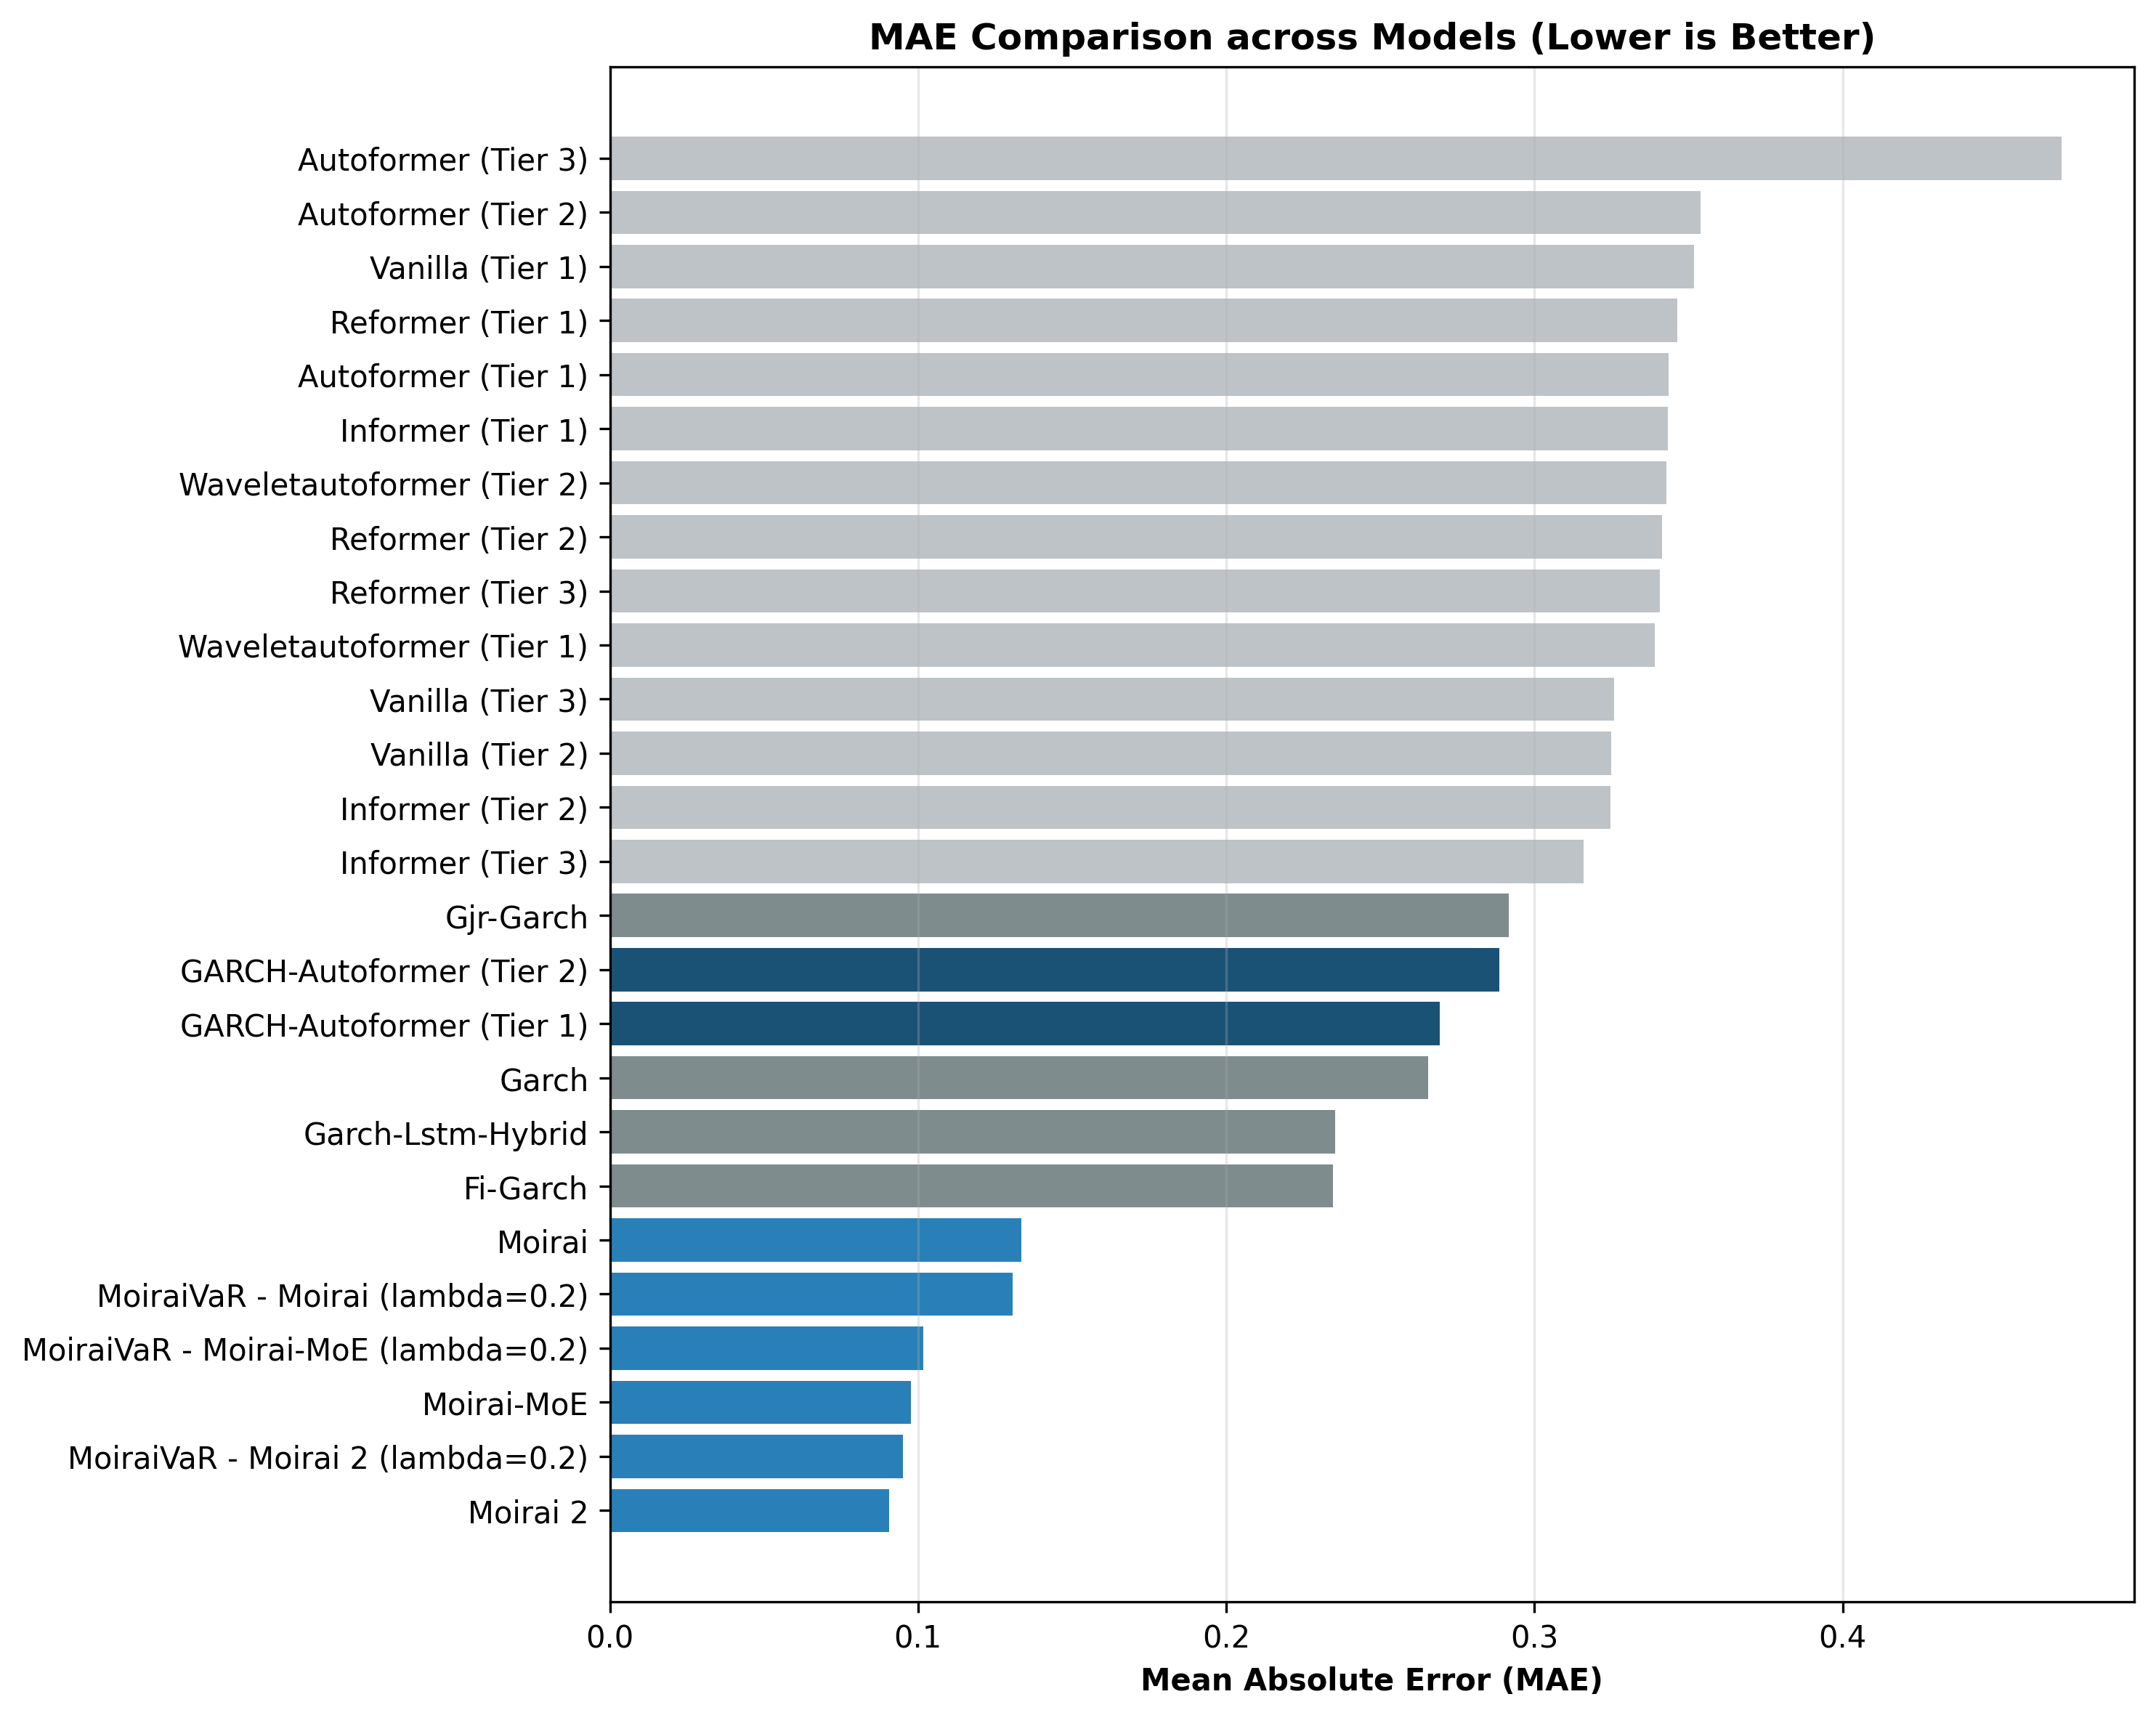
\includegraphics[width=\linewidth]{fig_mae_comparison}
\end{minipage}
\caption{Raw accuracy performance: Mean Squared Error (left) and Mean Absolute Error (right). Foundation models (Moirai and MoiraiVaR) achieve the lowest point-forecast errors.}
\label{fig:errors}
\end{figure}

\subsection{Sanity Gate and MCDM Ranking}

The Sanity Gate excluded 12 of the 26 configurations (including large Transformer tiers that suffered amplitude collapse despite low MSE). 
Under the \textbf{balanced (50:50)} scenario, Moirai-MoE and MoiraiVaR--Moirai~2 co-rank first, driven by the strong accuracy seen in Fig.~\ref{fig:errors}. 
Under the \textbf{risk-priority (30:70)} scenario, Autoformer (Tier 2) dominates the rankings, demonstrating that superior accuracy does not guarantee robust VaR coverage. The sensitivity to aggregation weights highlights the necessity of our multi-criteria approach for practical risk management.

\section{Conclusion}

We introduced GARCH-Autoformer and MoiraiVaR alongside a novel Forecast Sanity Gate and MCDM evaluation framework. Results confirm that standard accuracy metrics fail to detect degenerate tracking and do not align with tail-risk performance. The proposed risk-sensitive MCDM pipeline provides a rigorous mechanism for volatility model selection based on stakeholder priorities.

\begin{thebibliography}{10}

\bibitem{bollerslev1986}
Bollerslev, T.: Generalized autoregressive conditional heteroskedasticity.
J.\ Econom.\ \textbf{31}(3), 307--327 (1986)

\bibitem{bollerslev1987}
Bollerslev, T.: A conditionally heteroskedastic time series model for speculative prices and rates of return.
Rev.\ Econ.\ Stat.\ \textbf{69}(3), 542--547 (1987)

\bibitem{christoffersen1998}
Christoffersen, P.: Evaluating interval forecasts.
Int.\ Econ.\ Rev.\ \textbf{39}(4), 841--862 (1998)

\bibitem{demsar2006}
Dem\v{s}ar, J.: Statistical comparisons of classifiers over multiple data sets.
J.\ Mach.\ Learn.\ Res.\ \textbf{7}, 1--30 (2006)

\bibitem{gneiting2011}
Gneiting, T.: Making and evaluating point forecasts.
J.\ Am.\ Stat.\ Assoc.\ \textbf{106}(494), 746--762 (2011)

\bibitem{hwang1981}
Hwang, C.L., Yoon, K.: Multiple Attribute Decision Making: Methods and Applications.
Springer (1981)

\bibitem{kupiec1995}
Kupiec, P.: Techniques for verifying the accuracy of risk measurement models.
J.\ Deriv.\ \textbf{3}(2), 73--84 (1995)

\bibitem{liu2025}
Liu, Y., et al.: Moirai-MoE: empowering time series foundation models with sparse mixture of experts.
ICML (2025)

\bibitem{patton2011}
Patton, A.J.: Volatility forecast comparison using imperfect volatility proxies.
J.\ Econom.\ \textbf{160}(1), 246--256 (2011)

\bibitem{wu2021}
Wu, H., et al.: Autoformer: decomposition transformers with auto-correlation for long-term series forecasting.
NeurIPS (2021)

\bibitem{zeng2023}
Zeng, A., et al.: Are transformers effective for time series forecasting?
AAAI (2023)

\end{thebibliography}

\end{document}
